% -----------------------------------------------------------------------------
% Latex Template for Wuhan University Thesis
%
% Ack to Huang Zhenghua (http://aff.whu.edu.cn/huangzh/)
%
% Modified by iamywang
% Date: Jan 29, 2024
% Updated: Apr 13, 2024
% -----------------------------------------------------------------------------

\chapter{安全架构设计关键技术研究}\label{chap5}

\section{ZeRØ安全架构设计}

ZeRØ~\cite{ziad2021zero}提出了独特的内存指令和新颖的元数据编码方案来保护代码和数据指针,仅仅只需要微小的微架构变化。ZeRØ在SPEC CPU2017基准上的性能开销为零,VLSI测量显示了低功率和面积开销。

\begin{figure}[h!]
\centering
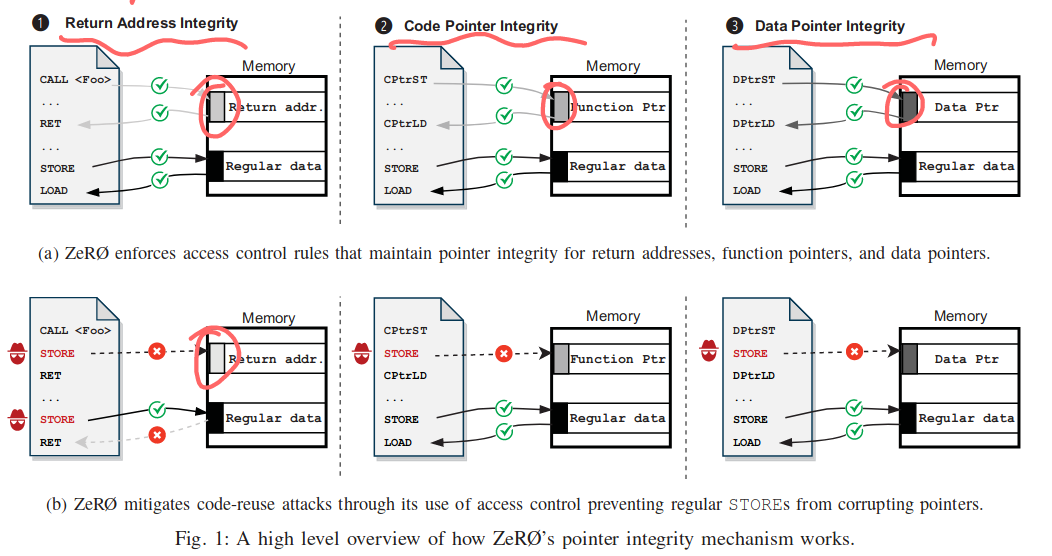
\includegraphics[width=0.8\linewidth]{fig5-1.png}
\caption{ZeRØ设计框架}
\label{fig5.1}
\end{figure}

\section{No-FAT安全架构设计}

No-FAT~\cite{ziad2021no}将内存分配大小(例如malloc大小)作为一个架构特征,来克服传统内存安全方法的许多棘手问题,例如与不安全软件的兼容性和显著的性能下降。No-FAT在SPEC CPU2017基准测试中产生了8\%的开销,VLSI测量显示了低功率和面积开销。

\begin{figure}[h!]
\centering
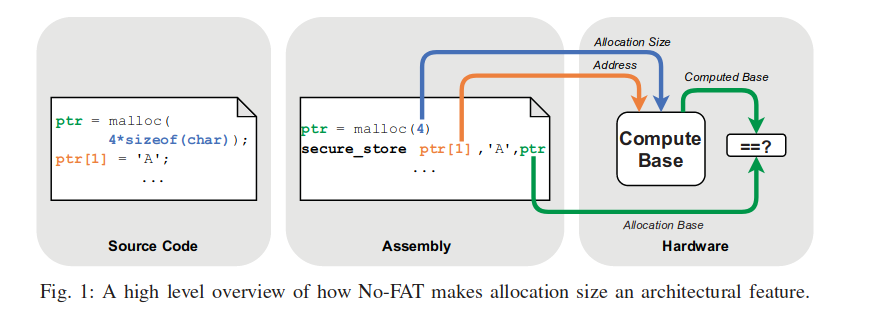
\includegraphics[width=0.8\linewidth]{fig5-2.png}
\caption{No-FAT设计框架}
\label{fig5.2}
\end{figure}